\documentclass[3p]{elsarticle}

\biboptions{super,sort&compress}

% Standard package includes for math, tables, and images
\usepackage{float}
\usepackage{enumitem}
\usepackage{subcaption}
\usepackage{amsmath}
\usepackage{booktabs}
\usepackage{graphicx}
\usepackage{url}
\usepackage{stfloats}
\usepackage{tabularx}
\usepackage{setspace}
\usepackage{xcolor}

% Font and layout improvements
\usepackage[T1]{fontenc}
\usepackage[utf8]{inputenc}
\usepackage{microtype}
\usepackage{inconsolata}
\usepackage{hyperref}

% Visible author placeholders -- remove all before submission
\newcommand{\authortodo}[1]{\textcolor{red}{\textbf{[TODO: #1]}}}

% TODO: previous value was "Engineering Fracture Mechanics" (left over from another manuscript)
\journal{[TODO: target journal]}

\begin{document}

\begin{frontmatter}

\title{Perovskite Solar Cell Performance Prediction with LLM-Derived Feature Augmentation under Leakage-Aware DOI Evaluation}

\author[1]{Sunraj Patel}
\author[1]{Shikhar Misra\corref{cor1}}

\cortext[cor1]{Corresponding author.}
\ead{shikharm@iitk.ac.in}

\address[1]{Department of Materials Science and Engineering, Indian Institute of Technology Kanpur, India 208016}


\begin{abstract}
Machine-learning (ML) models for perovskite solar cell (PSC) performance are increasingly trained on literature-derived databases such as the Perovskite Database Project (PDP), yet they are typically evaluated with record-level random splits, even though a single publication often contributes many closely related device records. Here, we develop a power conversion efficiency (PCE) prediction framework that augments PDP device and fabrication variables with composition-derived descriptors, curated material properties, and publication-level features extracted from 2,726 full-text articles with a locally served large language model (LLM). The framework is evaluated with repeated DOI-grouped holdout splits, so that every test publication is unseen during training. On unseen publications, the final model achieves an overall $R^2$ of $0.41 \pm 0.01$, MAE of $2.91 \pm 0.04$ and RMSE of $3.76 \pm 0.05$ percentage points, with $R^2$ of $0.37 \pm 0.02$ and $0.45 \pm 0.01$ for p-i-n and n-i-p architectures, respectively. Under matched model settings, material-property descriptors provide the largest gain over the database-only representation ($\Delta R^2 = +0.038$), and LLM-derived literature features give a further small but consistent improvement in every architecture subset and every error metric ($\Delta R^2 = +0.005$ to $+0.007$). Record-level random splitting overestimates $R^2$ by 0.17--0.24, with the largest inflation for the literature-augmented model, showing that publication-level evaluation is required for realistic performance estimates on literature-derived PSC data.
\authortodo{update all numbers after re-running with a DOI-disjoint validation split for early stopping (see Section 2.5.3)}
\end{abstract}

\begin{keyword}
Perovskite solar cells; Power conversion efficiency; Materials informatics; Large language models; Data leakage; SHAP interpretability.
\end{keyword}

\end{frontmatter}

% ---------------- INTRODUCTION ----------------
\section{Introduction}

Perovskite solar cells (PSCs) are promising photovoltaic devices whose performance depends on the absorber material, device architecture, and fabrication conditions. A typical planar PSC consists of five functional layers: a substrate, an electron transport layer (ETL), a perovskite absorber, a hole transport layer (HTL), and a metal electrode. As illustrated in Fig.~\ref{fig:psc_structures}, two widely used configurations are n-i-p and p-i-n, which differ in the relative positions of the ETL and HTL \cite{jung2015perovskite,zuo2016advances}. Under illumination, the perovskite absorber generates charge carriers, while the ETL and HTL selectively transport electrons and holes, respectively, towards the electrodes. Charge extraction and recombination, together with the properties of the constituent materials, influence the resulting photovoltaic performance \cite{jung2015perovskite,zuo2016advances}.

Power conversion efficiency (PCE) is the principal metric of PSC performance and represents the fraction of incident optical power converted into electrical power. The fill factor (FF) characterizes the shape of the current--voltage curve as the ratio of the maximum output power to the product of the open-circuit voltage and short-circuit current. These quantities are expressed as
\begin{equation}
\mathrm{PCE} =
\frac{V_{\mathrm{OC}}J_{\mathrm{SC}}\mathrm{FF}}{P_{\mathrm{in}}}
\times 100\%,
\end{equation}
and
\begin{equation}
\mathrm{FF} =
\frac{V_{\mathrm{MPP}}J_{\mathrm{MPP}}}
{V_{\mathrm{OC}}J_{\mathrm{SC}}},
\end{equation}
where $V_{\mathrm{OC}}$ and $J_{\mathrm{SC}}$ denote the open-circuit voltage and short-circuit current density, respectively; $V_{\mathrm{MPP}}$ and $J_{\mathrm{MPP}}$ are the voltage and current density at the maximum power point; and $P_{\mathrm{in}}$ is the incident optical power density \cite{zuo2016advances}. The dependence of PCE on multiple interacting material, architectural, and processing variables makes systematic device optimization challenging. Machine learning (ML) offers a data-driven approach to identifying these relationships and exploring combinations of experimentally reported parameters that would be difficult to investigate exhaustively through conventional trial-and-error approaches \cite{odabasi2019performance,bansal2023machine,li2019predictions,liu2022machine,gok2022predicting}.

\begin{figure}[t]
    \centering
    \includegraphics[width=0.95\textwidth]{figures/device_structure.png}
    \caption{Example device structure for a (a) n-i-p and (b) p-i-n perovskite solar cell.}
    \label{fig:psc_structures}
\end{figure}

The availability of large experimental databases has enabled ML models to be developed using combinations of material, device, and process information. The Perovskite Database Project (PDP) provides an open-access collection of PSC data covering material compositions, device structures, fabrication conditions, and photovoltaic characteristics \cite{jacobsson2022open}. Roberts et al. developed an open-source ML pipeline using the PDP and evaluated XGBoost, artificial neural networks, and Gaussian process regression for predicting short-circuit current density. Their XGBoost model achieved a test $R^2$ of 0.35 and an RMSE of $3.58$ mA cm$^{-2}$, while their analysis highlighted the importance of data cleaning, feature encoding, and reproducible workflows \cite{roberts2024machine}. Other device-level studies have similarly examined the influence of descriptor selection and dataset characteristics on predictive performance \cite{sala2023assessing}.

Fukasawa et al. examined the representation of material and process information specifically for PCE prediction using the PDP \cite{fukasawa2024effectiveness}. Starting with 42,459 records, they curated the dataset to obtain 36,937 records with 248 material- and process-related variables. Their results demonstrated that incorporating process information improved prediction compared with using perovskite composition alone. Under a conventional random train--test split, their best feature representation achieved a test $R^2$ of 0.7177; however, evaluation on 294 newly registered records yielded an $R^2$ of 0.45 and an MAE of 3.20\% \cite{fukasawa2024effectiveness}. They also identified substantial data degeneracy, with 6,446 unique degenerate points corresponding to 20,695 feature vectors, indicating that distinct experimental records can have identical feature representations despite exhibiting different PCE values.

The distinction between interpolation within an existing dataset and generalization to new groups of observations is also recognized in the broader materials-informatics and machine-learning literature. Meredig et al. introduced leave-one-cluster-out cross-validation to examine how evaluation strategies affect estimates of model performance for materials discovery, emphasizing that conventional random validation may not adequately represent extrapolative use cases \cite{meredig2018cluster}. More broadly, Kapoor and Narayanan documented data leakage as a recurring source of overoptimistic findings and reproducibility problems across scientific machine-learning applications \cite{kapoor2023leakage}. These studies establish that evaluation should reflect the intended generalization setting and the dependence structure of the data. In literature-compiled PSC datasets, publication DOI provides a practical grouping variable for assessing performance on papers excluded from training. Our work applies this principle to PCE prediction and quantifies how the estimated performance and feature-tier comparisons change when publication-level overlap is removed.

The literature-derived nature of PSC databases raises a further concern about model evaluation. Multiple devices reported in the same publication may share material selections, fabrication procedures, device architectures, and measurement conditions, making record-level independence an assumption that requires scrutiny. Roberts et al. documented substantial duplication of device configurations in the Perovskite Database Project (PDP) and addressed it by averaging target values within duplicate groups \cite{roberts2024machine}. Fukasawa et al. reported a reduction in predictive performance from \(R^2=0.7177\) under their conventional evaluation to \(R^2=0.45\) with an MAE of \(3.20\) percentage points on 294 newly registered records \cite{fukasawa2024effectiveness}. This result provides prior evidence that performance estimates can be sensitive to the evaluation set and the distribution of newly reported devices. However, the newly registered-record evaluation was relatively small and was not presented as a systematic DOI-grouped cross-validation protocol. Group-aware validation and data-leakage analysis are established methodological concerns in machine learning; the contribution here is to apply explicit DOI-grouped evaluation to the PDP-based PCE prediction task and quantify its effect under matched feature representations and model settings. Such evaluation prevents records sharing a DOI from appearing in both training and test partitions, providing a direct assessment of generalization to publications excluded from training.


In this work, we develop a literature- and material-augmented ML framework for predicting PSC PCE from the PDP, and evaluate it at the publication level. The contributions are twofold.
\begin{enumerate}[label=(\roman*)]
\item \textbf{Feature augmentation.} We combine PDP device and fabrication variables with composition-derived descriptors, curated layer-resolved material properties, and publication-level features extracted from the full text of 2,726 articles using a locally served LLM. Nested feature-tier ablations under a fixed model configuration show that material-property descriptors provide the largest gain over the database-only representation, and that LLM-derived literature features give a further small but consistent improvement across both architectures and all error metrics.
\item \textbf{Publication-level evaluation.} We evaluate PCE prediction using repeated DOI-grouped holdout splits and compare the results with record-level random splitting under matched feature representations and model configurations. Building on earlier evidence that performance can decline when models are evaluated on newly registered PSC records, this analysis quantifies the sensitivity of predictive performance to publication-level separation and examines how that sensitivity varies across the three feature tiers.
\end{enumerate}

SHAP-based interpretation is further used to characterize the features associated with model predictions in the n-i-p and p-i-n architectures. The overall workflow is summarized in Fig.~\ref{fig:ml_workflow}.

\begin{figure}[t]
    \centering
    \includegraphics[width=\textwidth]{figures/ml_pipeline.png}
    \caption{Overview of the machine-learning workflow for perovskite solar-cell power conversion efficiency (PCE) prediction. The Perovskite Database Project provided unique DOIs, from which full-text PDFs were retrieved, which were converted to Markdown. Subsequently structured JSON files were generated through large language model (LLM)-based extraction. The resulting literature-derived features were integrated with structured database descriptors at the DOI level, followed by publication-grouped model evaluation using CatBoost and model interpretation using SHAP.
    \authortodo{regenerate panels 2 and 6: panel 6 states ``XGBoost, 3,000 trees, depth 12'' (Methods: single CatBoost, depth 8, 1,500 iterations) and subset sizes $\approx$42K/15K/27K (actual 41,107/12,684/28,340); panel 2 states $\approx$90 device features (Table 2: 30) and implies all 2,817 materials received properties (only those with frequency $\geq$100)}}
    \label{fig:ml_workflow}
\end{figure}

% ---------------- METHODOLOGY ----------------
\section{Methods}

\subsection{Data Preparation}

\subsubsection{Dataset Description}

The Perovskite Database Project (PDP) is an open-access repository of experimentally reported perovskite solar cell (PSC) data, encompassing material compositions, device architectures, fabrication procedures, and photovoltaic characteristics \cite{jacobsson2022open}. The database export used in this study contained 43,398 device records, associated with 7,499 unique DOIs, and 410 columns. These records comprise heterogeneous data types, including categorical descriptions of functional layers, perovskite compositions, numerical device parameters, and fabrication-related variables. Previous PDP-based studies have demonstrated that appropriate data selection, cleaning, and representation are important for developing predictive models from these heterogeneous records \cite{roberts2024machine,fukasawa2024effectiveness}.

Five fields were initially extracted to construct the layer-resolved material representation: \texttt{ETL\_stack\_sequence}, \texttt{HTL\_stack\_sequence}, \texttt{Perovskite\_composition\_short\_form}, \texttt{JV\_default\_PCE}, and \texttt{Cell\_architecture}. These fields describe the electron transport layer (ETL), hole transport layer (HTL), perovskite composition, experimentally reported power conversion efficiency (PCE), and device architecture, respectively. The PCE field was renamed \texttt{final\_pce} for consistency throughout the processing pipeline, while the architecture field was retained for pooled modelling and architecture-specific analysis. This five-column extract was an intermediate representation for material processing rather than the complete predictor matrix; additional device and fabrication variables were retained from the original database for subsequent feature construction. Publication metadata, including DOI identifiers and author information, were excluded from the predictive feature set, while DOI identifiers were retained separately for linking records to the literature corpus and defining publication-level data partitions.

\subsubsection{Layer-Stack Parsing and Material Catalogue}

The material-stack descriptions in the PDP are stored as strings containing multiple materials or sequential layers, with vertical bars (\texttt{|}) delimiting successive entries. These strings were parsed into position-indexed fields, such as \texttt{ETL\_1}, \texttt{HTL\_1}, and \texttt{Perovskite\_1}, making the constituent materials independently accessible. The resulting representation accommodated up to seven ETL entries, three HTL entries, and five perovskite-layer entries. Where an entry contained multiple semicolon-separated materials, the individual materials were expanded into separate fields while preserving the recorded stack order. Material identifiers were also normalized by consolidating selected naming variants into common identifiers, facilitating consistent matching across device records.

A catalogue of unique standardized material identifiers was subsequently constructed from the parsed ETL, HTL, and perovskite fields. The catalogue contained 2,817 unique material identifiers, and the occurrence frequency of each identifier was calculated by counting its appearances across the parsed stack fields. This catalogue provided a common reference for material-level property retrieval and the construction of layer-specific descriptors (Section~\ref{sec:matprop}). The parsed identifiers were used for property lookup and were not themselves supplied to the models as categorical predictors.

\subsection{Literature Corpus Construction}

\subsubsection{DOI Identification and Full-Text Retrieval}

To enrich the structured device database with information from the original experimental literature, publication identifiers were extracted from the \texttt{Ref\_DOI\_number} field of the PDP. In total, 7,499 unique DOIs were identified across the 43,398 device records (7,371 after the record filtering described in Section~\ref{sec:integration}). These identifiers were used to drive an automated full-text retrieval workflow, with retrieved documents associated with their corresponding DOIs to maintain traceability throughout subsequent processing. \authortodo{state the retrieval source(s) and access route, e.g.\ open-access resolver, publisher text-and-data-mining APIs, institutional subscription; add a data availability statement on what can be shared}. The retrieval stage yielded 3,299 PDF documents. As full-text availability and successful retrieval varied across publications, the resulting corpus represented the subset of identified publications for which PDF documents were obtained.

\subsubsection{PDF Conversion and LLM-Based Information Extraction}

The retrieved PDF documents were converted individually into Markdown using OpenDataLoader PDF, an open-source PDF parsing tool designed to produce machine-readable representations of document content and structure \cite{opendataloaderpdf}. This conversion yielded 3,141 Markdown documents from the 3,299 retrieved PDFs. The resulting files provided a text-based representation of each publication for subsequent processing by a large language model (LLM).

Each Markdown document was supplied individually to a locally served Qwen3.5-9B model \authortodo{replace citation with the Qwen model technical report; verify exact model name and version} using a predefined system prompt, multi-shot prompting with representative input--output examples \cite{brown2020fewshot}, and a structured JSON schema to guide consistent information extraction. The extraction procedure was designed to identify reported materials and their functional classifications, together with available material properties, units, uncertainties, and measurement methods. Fabrication-related information, including deposition techniques, spin-coating parameters, annealing conditions, and processing environments, was also extracted where reported. Photovoltaic performance information was collected separately, with champion and average performance values distinguished where possible. The resulting structured outputs retained their association with the source DOI for subsequent paper-level feature construction.

The individual extraction outputs were consolidated into a combined JSON representation and subsequently organized into DOI-indexed JSON files. This process yielded 2,835 structured paper records. These records served as the intermediate representation for downstream feature construction, in which the extracted information was normalized and converted into a consistent set of publication-level descriptors for integration with the device-level database.

\authortodo{extraction validation: precision/recall against a hand-annotated subset of $N$ papers for key fields (materials and layer roles, deposition method, annealing temperature/time, thicknesses); hallucination rate; per-field coverage across the 2,835 records; reasons for attrition 3,299 $\rightarrow$ 3,141 $\rightarrow$ 2,835 $\rightarrow$ 2,726 matched DOIs}

\subsubsection{DOI-Level Feature Construction}

The structured JSON records were parsed to construct a tabular dataset of publication-level features for integration with the device database. An initial, broader feature representation was developed and subsequently refined to retain information relevant to PSC materials and fabrication. The feature-construction procedure used recursive traversal of nested JSON objects to retrieve property values and associated units, together with normalization of synonymous field names and material-type labels. This harmonization enabled information expressed using different terminology across publications to be mapped to consistent feature definitions.

The resulting features represented material properties and fabrication conditions reported in the source literature, including layer-specific properties, deposition parameters, annealing conditions, and available processing-environment information. Material and layer assignments were resolved using standardized material classifications and bounded pattern matching to reduce false matches between similar material names. Layer-specific descriptors were retained separately rather than averaging properties across different functional layers. In addition to these material and processing descriptors, the table includes extraction-level descriptors, such as the number of numerical values recovered from a paper, which summarize how completely a publication reports its experimental details. Bibliographic metadata, including author names, journal names, and publication year, were excluded.

The final DOI-level feature table contained one row per successfully processed publication. These features represented information extracted from the associated research paper and were therefore defined at the publication level, rather than as independent measurements for every device reported in that paper. The table was subsequently linked to the device-level dataset by DOI.


\subsection{Feature Engineering}

\subsubsection{Composition-Derived Descriptors}

Composition-derived descriptors were constructed to represent the elemental and ionic composition of the perovskite absorber numerically. These features included the fractions of constituent ions at the A, B, and X sites and corresponding ion counts.

In addition to the site-specific composition descriptors, the feature set included composition-derived descriptors representing the average atomic mass and ionic radius of the perovskite absorber. The feature \texttt{Perovskite\_avg\_atomic\_mass} was calculated as a stoichiometric average of the atomic masses of the constituent elements. For a composition containing \(k\) constituent elements, this descriptor is defined as

\[
\overline{M}=\frac{\sum_{i=1}^{k} n_i M_i}{\sum_{i=1}^{k} n_i},
\]

where \(n_i\) is the stoichiometric coefficient of element \(i\) in the composition and \(M_i\) is its atomic mass. Consequently, the descriptor represents the average atomic mass weighted by the elemental stoichiometry rather than an unweighted average of the constituent atomic masses. It provides a compact numerical representation of compositional differences that can be used alongside the individual site-fraction and ion-count descriptors.

The feature \texttt{Perovskite\_avg\_radius} represents an average ionic-radius descriptor for the perovskite composition. It summarizes the ionic sizes associated with the constituent species and complements the site-specific composition descriptors by providing a scalar representation of the composition's characteristic ionic size. The resulting values depend on the ionic-radius reference data and the weighting procedure used during feature construction.

The feature \texttt{perovskite\_octahedral\_factor} represents a geometric descriptor of the perovskite composition. For an idealized \(ABX_3\) composition, the octahedral factor is defined as

\[
\mu=\frac{r_B}{r_X},
\]

where \(r_B\) and \(r_X\) are the ionic radii of the B-site cation and X-site anion, respectively. This ratio characterizes the relative sizes of the ions forming the \(BX_6\) octahedral framework. For mixed compositions, its calculation depends on how the effective B-site and X-site ionic radii are obtained from the constituent species. The octahedral factor was included as a composition-derived predictor; its inclusion does not, by itself, establish structural stability or a causal relationship with power conversion efficiency.

\subsubsection{Material-Property Augmentation}
\label{sec:matprop}

A separate material-property reference dataset was curated for standardized material identifiers with an occurrence frequency of at least 100 across the parsed ETL, HTL, and perovskite stacks. Available electronic and physicochemical properties were compiled from published literature and, where applicable, retrieved through the Materials Project database \cite{jain2013materialsproject}. These values represent general material-level reference properties rather than measurements reported for the specific PSC devices in which the materials appeared. Property availability was heterogeneous, and not every material had a complete set of descriptors.

The curated property catalogue included band gap, highest occupied molecular orbital (HOMO) energy, lowest unoccupied molecular orbital (LUMO) energy, electron mobility, hole mobility, dielectric constant, and material classification, together with the material identifier and occurrence frequency. Source references were associated with the curated values to support traceability.

For each device, property lookup was performed separately for the ETL, HTL, and perovskite layers. Within each layer family, the recorded material entries were traversed in their original order, and the first available non-missing value was assigned for each property. This procedure produced descriptors such as \texttt{ETL\_band\_gap}, \texttt{HTL\_HOMO}, and \texttt{Perovskite\_dielectric\_constant}. Because the lookup was performed independently for each property, the material supplying one descriptor was not necessarily the same material supplying another descriptor for a given layer family. Missing property values were retained during this stage and handled during model feature preparation.

\subsubsection{PDP-Derived Process and Device Features}

The composition descriptors were combined with relevant device and fabrication variables retained from the original PDP export. These variables included available layer-thickness information, deposition methods and solvents, annealing conditions, and device-related flags. Because the parsed material identifiers were not used as predictors, this database-level representation ($t_1$, Section~\ref{sec:tiers}) contains no explicit information on which transport-layer materials were used; that information enters the model only through the material-property descriptors of $t_2$.

\subsubsection{LLM-Derived Literature Features}

The DOI-level feature table was used to augment the device-level representation with information extracted from the associated research papers. Paper-level features were not treated as device-specific experimental measurements; instead, they provided publication-level context derived from the reported literature. The feature-construction process normalized aliases and functional classifications before producing the final DOI-level table, allowing the same feature definitions to be applied consistently across publications. Photovoltaic outcome fields extracted during literature processing were not used as model predictors. \authortodo{list all 44--46 LLM-derived features with definitions in the SI}

\subsection{Data Integration, Filtering and Feature Tiers}
\label{sec:integration}

The structured device-level feature table and the DOI-level literature feature table were integrated using the publication DOI as the join key. DOI strings were normalized by converting them to lowercase and removing leading and trailing whitespace before matching. A left join was performed from the device-level table to the DOI-level feature table, retaining the device records even when a corresponding literature-feature record was unavailable. Missing paper-level features arising from unsuccessful retrieval, incomplete extraction, or unmatched DOI identifiers were preserved as missing values for subsequent model preparation.

The initial PDP export contained 43,398 records associated with 7,499 unique DOIs. We excluded 1,002 records with missing target values and a further 1,289 records with reported PCE below 1.0\%, giving 41,107 records from 7,371 unique DOIs (Table~\ref{tab:dataset}). Of these, 28,340 records were n-i-p and 12,684 were p-i-n devices; the remaining 83 records have other or unspecified architectures and were used only in the pooled model. \authortodo{the filtered set contains PCE values up to 36.2\% (training maximum 30.0\%), above the certified single-junction perovskite record ($\approx$27\%); check the PDP illumination and tandem fields and exclude tandem and non-AM1.5G records, or justify retaining them} The DOI was used exclusively as a record-linkage and grouping variable and was never a predictor. The 232 filtered records without a DOI were treated as a single group during splitting. Free-text columns and columns with more than 80\% missing values were removed. Numerical features with missing entries were median-imputed and accompanied by a binary missingness indicator (suffix \texttt{\_na}), and missing categorical features were assigned the label ``unknown''. The complete list of predictor columns for each tier is given in the Supplementary Information (Table~S1).

\begin{table}[t]
\centering\small
\caption{Summary of the dataset used for modelling.}
\label{tab:dataset}
\begin{tabular}{lr}
\toprule
Quantity & Value \\
\midrule
Records in PDP export (unique DOIs) & 43,398 (7,499) \\
Removed: missing PCE & 1,002 \\
Removed: PCE $<$ 1.0\% & 1,289 \\
Records after filtering (unique DOIs) & 41,107 (7,371) \\
\quad n-i-p / p-i-n / other architecture & 28,340 / 12,684 / 83 \\
\quad Records without DOI & 232 \\
Records with LLM-derived literature features (unique DOIs) & 14,896 (2,726) \\
PCE after filtering: mean, median, range (\%) & 12.4, 13.0, 1.0--36.2 \\
Records per DOI: median, maximum & 4, 127 \\
\bottomrule
\end{tabular}
\end{table}

\subsection{Machine Learning Models and Evaluation}

\subsubsection{Prediction task and feature tiers.}
\label{sec:tiers}
We formulated PCE prediction as a supervised regression task, with experimentally reported PCE as the target. Three nested feature tiers were defined (Table~\ref{tab:tiertable}): the PDP database representation ($t_1$), comprising device architecture, layer deposition and fabrication variables and composition-derived descriptors; $t_1$ augmented with material-property descriptors ($t_2$); and $t_2$ further augmented with LLM-derived literature features ($t_3$). Each tier was evaluated on the pooled dataset and separately on the p-i-n and n-i-p subsets, which were modelled independently.

\begin{table}[t]
\centering\small
\caption{Feature tiers. Feature counts refer to the pooled model; the p-i-n and n-i-p models contain 77/179/225 and 75/177/221 features for $t_1$/$t_2$/$t_3$, respectively.}
\label{tab:tiertable}
\begin{tabular}{llrl}
\toprule
Feature group & Tier & No. of features & Content \\
\midrule
Process & $t_1$ & 21 & Deposition methods, annealing, layer thickness \\
Device & $t_1$ & 9 & Architecture and device flags \\
Composition & $t_1$ & 47 & A-, B- and X-site ion fractions and counts \\
Material properties & $t_2$ & 102 & Band gap, HOMO/LUMO, mobility, etc. \\
Literature (LLM) & $t_3$ & 44 & Paper-level features from LLM extraction \\
\midrule
Total & $t_1$ / $t_2$ / $t_3$ & 77 / 179 / 223 & \\
\bottomrule
\end{tabular}
\end{table}

\subsubsection{Model training.}
\label{sec:models}
Models were trained with CatBoost \cite{prokhorenkova2018catboost}, using its native handling of the categorical variables (architecture and the deposition methods). To ensure a controlled comparison across feature tiers, all three tiers used a single CatBoost regressor with the same fixed hyperparameter configuration: depth 8, learning rate 0.05, and at most 1,500 iterations (Table~\ref{tab:config}). The only difference between tiers is the predictor set, so the tier comparisons are feature ablations rather than comparisons between model architectures or hyperparameter settings. The complete hyperparameter set is given in the Supplementary Information.

\begin{table}[t]
\centering\small
\caption{Model configuration for each feature tier (full hyperparameters in the Supplementary Information).}
\label{tab:config}
\begin{tabular}{llll}
\toprule
Tier & Model & Depth / learning rate & Max. iterations \\
\midrule
$t_1$, $t_2$, $t_3$ & CatBoost, single model & 8 / 0.05 & 1,500 \\
\bottomrule
\end{tabular}
\end{table}

\subsubsection{Evaluation protocol with a DOI-disjoint validation set.}
To evaluate generalization to previously unseen publications, we used five repeated DOI-grouped holdout splits generated with \texttt{GroupShuffleSplit} (test fraction 0.2 of DOIs, random seed 42), so that records sharing a DOI were always assigned to the same partition (Table~\ref{tab:protocol}). Within each training partition, a validation subset, also DOI-disjoint from the remainder of the training data and from the test partition, was used for early stopping; the test partition was used only for final evaluation. \authortodo{the released scripts currently early-stop on the test partition; re-run with a DOI-disjoint validation split, then update all reported numbers, the validation fraction, and Table~\ref{tab:protocol}} The absence of DOI overlap between training and test partitions was verified for every split. Because repeated group-shuffle splits may have overlapping test sets, the evaluation is a repeated DOI-grouped holdout evaluation rather than mutually exclusive five-fold cross-validation. Predictive performance was calculated independently for each split and is reported as the mean and standard deviation across the five runs. Record-wise random splitting (five splits, test fraction 0.2, seed 42) was used with the same models only as a comparison protocol (Section~\ref{sec:splits}).

\begin{table}[t]
\centering\small
\caption{Data-splitting protocol.}
\label{tab:protocol}
\begin{tabular}{ll}
\toprule
Item & Setting \\
\midrule
Grouping variable & Publication DOI \\
Splitter & \texttt{GroupShuffleSplit}, 5 repeats, seed 42 \\
Test fraction & 0.2 of DOIs (about 1,475 DOIs, 8,300 records) \\
Training set (pooled) & about 5,900 DOIs, 32,800 records \\
Validation set & DOI-disjoint subset of the training partition; used for early stopping only \authortodo{fraction} \\
DOI overlap, train versus test & Zero in every split \\
Comparison protocol & Record-wise \texttt{ShuffleSplit}, 5 repeats, 0.2, seed 42 \\
Reported statistics & Mean $\pm$ s.d. over the five splits \\
\bottomrule
\end{tabular}
\end{table}

\subsubsection{Performance metrics.}
Predictive performance was assessed using the coefficient of determination ($R^2$), mean absolute error (MAE), and root mean squared error (RMSE), calculated by comparing experimentally reported PCE values, $y_i$, with predictions, $\hat{y}_i$, for the $N$ records in each held-out test partition:
\begin{equation}
R^2 =
1-\frac{\sum_{i=1}^{N}(y_i-\hat{y}_i)^2}
{\sum_{i=1}^{N}(y_i-\bar{y})^2},
\end{equation}
\begin{equation}
\mathrm{MAE} =
\frac{1}{N}\sum_{i=1}^{N}|y_i-\hat{y}_i|,
\end{equation}
\begin{equation}
\mathrm{RMSE} =
\sqrt{\frac{1}{N}\sum_{i=1}^{N}(y_i-\hat{y}_i)^2},
\end{equation}
where $\bar{y}$ is the mean experimentally reported PCE in the corresponding test partition. MAE and RMSE are expressed in PCE percentage points. The coefficient of determination measures performance relative to a constant-mean reference, whereas MAE and RMSE quantify absolute prediction errors, with RMSE assigning greater weight to large deviations.

\subsection{Feature Importance and Model Interpretation}

SHAP (Shapley additive explanations) was used to interpret the fitted CatBoost models and quantify the contributions of individual predictors to PCE predictions \cite{shappaper}. SHAP values were computed with \texttt{TreeExplainer} for a random sample of 1,500 held-out records from the first DOI-grouped split, using the CatBoost model trained for $t_3$. Global feature importance was assessed using mean absolute SHAP values. The analysis was conducted for the pooled dataset and the separate p-i-n and n-i-p models, and features were aggregated into the groups of Table~\ref{tab:tiertable} to compare group-level contributions. Because the p-i-n and n-i-p models were trained on different records, differences between their rankings describe what each model learned rather than different physical effects in the two architectures.

% ---------------- RESULTS AND DISCUSSION ----------------
\section{Results and Discussion}

\subsection{Generalization to unseen publications}

We first compared the gradient-boosted tree model (CatBoost) with Gaussian process regression (GPR) and a multilayer perceptron (ANN) on the first DOI-grouped split, using identical features and the same 8{,}395 test records (Table~\ref{tab:models}). The tree model achieved the lowest MAE and RMSE and the highest $R^2$ ($R^2 = 0.403e$ and RMSE $= 3.81$, versus $0.294$ and $4.14$ for GPR and $0.175$ and $4.48$ for ANN). We therefore used CatBoost for all subsequent analyses.

\begin{table}[t]
\centering\small
\caption{Model comparison on the first DOI-grouped split ($n = 8,395$ test records) using the $t_3$ features.}
\label{tab:models}
\begin{tabular}{lccc}
\toprule
Model & $R^2$ & MAE & RMSE \\
\midrule
CatBoost & 0.403 & 2.92 & 3.81 \\
GPR      & 0.294 & 3.26 & 4.14 \\
ANN      & 0.175 & 3.44 & 4.48 \\
\bottomrule
\end{tabular}
\end{table}

The predicted-PCE distributions (Fig.~\ref{fig:dist_trio}) show that all three models compress predictions toward the centre of the experimental distribution, most strongly for the GPR, whose predictions concentrate near 11--13\%. Two factors account for the under-representation of high-efficiency devices. First, high PCE values are rare: only 270 of the 8,395 test records exceed 20\%. Regressors trained with a squared-error loss estimate conditional means, so with $R^2 \approx 0.4$ the spread of the predictions is approximately $\sqrt{0.4}\approx 0.63$ times that of the experimental values. The maximum predicted PCE was 20.9\% for CatBoost and 20.3\% for the GPR, and test devices with PCE $\geq$ 20\% were under-predicted by 4.6 percentage points on average. Second, the high-PCE tail of the test set is thin: the histogram axes in Fig.~\ref{fig:dist_trio} extend to the 99.5th percentile, beyond which only a few dozen records lie, including a single 36.2\% record from one publication (the training maximum was 30.0\%).

\begin{figure}[t]
\centering
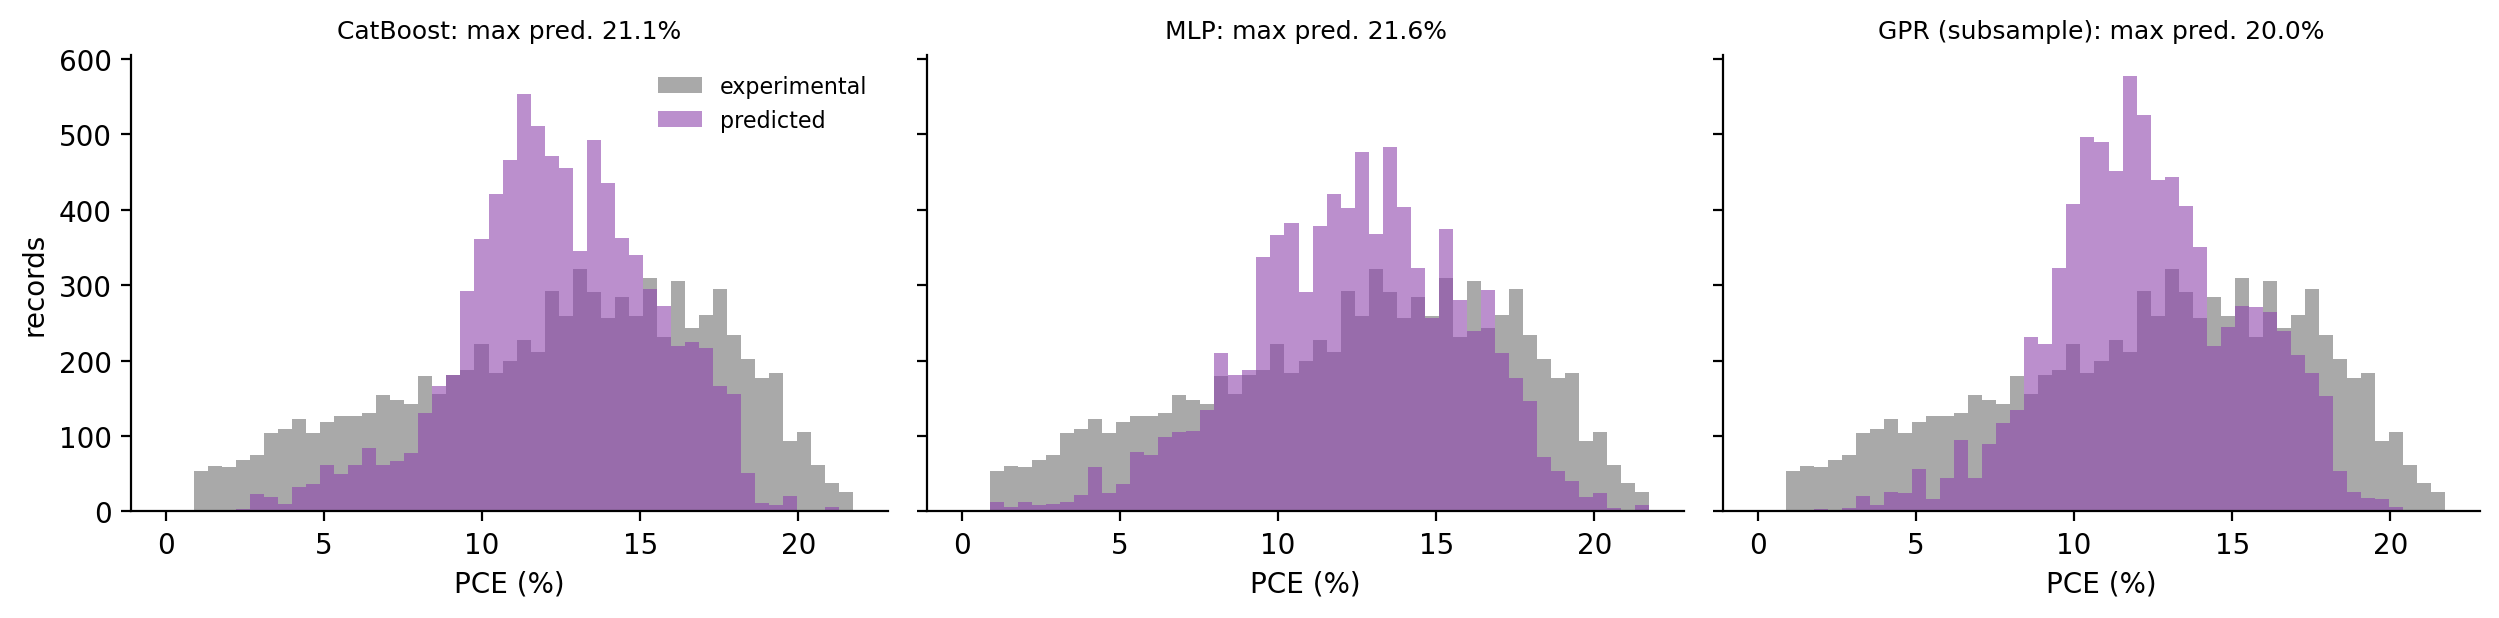
\includegraphics[width=\textwidth]{figures/fig_pce_dist_trio.png}
\caption{Distribution of experimental and predicted PCE on the first DOI-grouped split for (a) CatBoost, (b) Gaussian process regression and (c) the neural network. Axes extend to the 99.5th percentile of experimental PCE; 270 of the 8,395 test records exceed 20\%.}
\label{fig:dist_trio}
\end{figure}

The final models were evaluated on five repeated DOI-grouped holdout splits in which 20\% of publications were held out for testing (Table~\ref{tab:tiers}, Fig.~\ref{fig:tiers}). With all features ($t_3$), the pooled model reached $R^2 = 0.413 \pm 0.011$, MAE $= 2.91 \pm 0.04$ and RMSE $= 3.76 \pm 0.05$ percentage points on publications it had not seen. Performance differed by architecture: $R^2$ was $0.452 \pm 0.014$ for n-i-p and $0.365 \pm 0.020$ for p-i-n devices, whereas MAE (2.91 and 2.87) and RMSE (3.71 and 3.70) were nearly identical. Because $R^2$ depends on the variance of PCE within each subset, the higher n-i-p $R^2$ should not be read as n-i-p devices being intrinsically easier to predict.

\begin{table}[t]
\centering\small
\caption{Performance across feature tiers using the same CatBoost configuration (Table~\ref{tab:config}) under repeated DOI-grouped holdout evaluation (mean $\pm$ s.d. over five splits; MAE and RMSE in PCE percentage points).}
\label{tab:tiers}
\begin{tabular}{llrccc}
\toprule
Subset & Feature tier & $N$ & $R^2$ & MAE & RMSE \\
\midrule
Overall & Database only ($t_1$) & 41,107 & $0.370 \pm 0.011$ & $3.045 \pm 0.031$ & $3.895 \pm 0.051$ \\
Overall & + material ($t_2$) & 41,107 & $0.409 \pm 0.012$ & $2.923 \pm 0.034$ & $3.774 \pm 0.055$ \\
Overall & + material + LLM ($t_3$) & 41,107 & $0.413 \pm 0.011$ & $2.908 \pm 0.036$ & $3.759 \pm 0.046$ \\
\midrule
p-i-n & Database only ($t_1$) & 12,684 & $0.293 \pm 0.027$ & $3.083 \pm 0.093$ & $3.901 \pm 0.101$ \\
p-i-n & + material ($t_2$) & 12,684 & $0.358 \pm 0.022$ & $2.895 \pm 0.099$ & $3.717 \pm 0.102$ \\
p-i-n & + material + LLM ($t_3$) & 12,684 & $0.365 \pm 0.020$ & $2.871 \pm 0.081$ & $3.696 \pm 0.086$ \\
\midrule
n-i-p & Database only ($t_1$) & 28,340 & $0.412 \pm 0.011$ & $3.034 \pm 0.047$ & $3.843 \pm 0.057$ \\
n-i-p & + material ($t_2$) & 28,340 & $0.446 \pm 0.010$ & $2.925 \pm 0.034$ & $3.731 \pm 0.034$ \\
n-i-p & + material + LLM ($t_3$) & 28,340 & $0.452 \pm 0.014$ & $2.906 \pm 0.033$ & $3.710 \pm 0.038$ \\
\bottomrule
\end{tabular}
\end{table}

\begin{figure}[t]
\centering
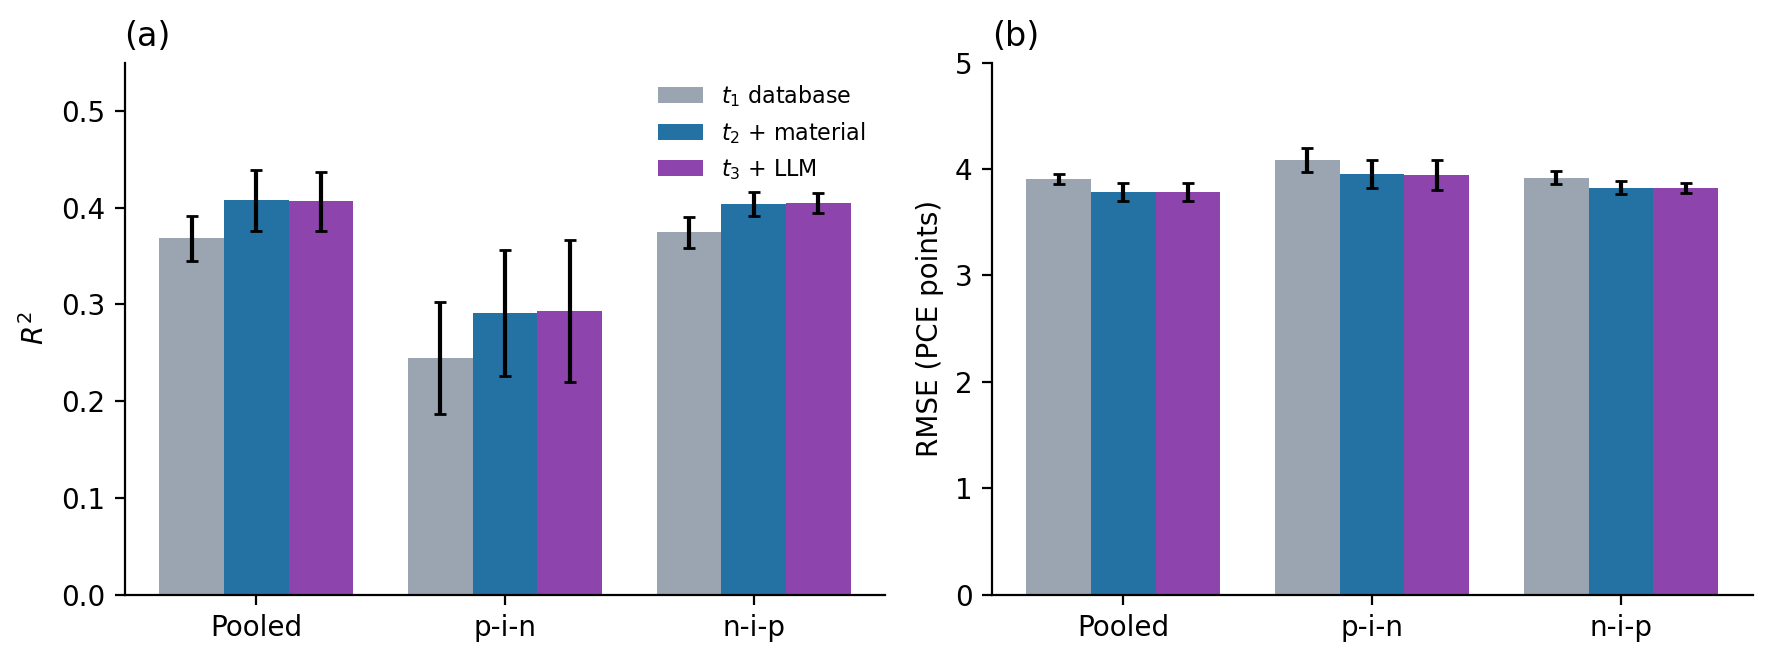
\includegraphics[width=\textwidth]{figures/fig_feature_tiers.png}
\caption{Effect of feature tier on prediction of unseen publications. (a) $R^2$ and (b) RMSE (mean $\pm$ s.d. over five DOI-grouped holdout splits). Adding material-property descriptors ($t_2$) improves all metrics; adding LLM-derived literature features ($t_3$) gives a further small improvement in mean $R^2$ and RMSE in all three subsets.}
\label{fig:tiers}
\end{figure}

\subsection{Effect of the evaluation protocol}
\label{sec:splits}

The evaluation protocol had a large influence on measured performance. Table~\ref{tab:split} and Fig.~\ref{fig:split} compare record-level random splitting with DOI-grouped splitting across the three feature tiers, using the same models, dataset, and filtering criteria. In a record-level random split, devices from the same publication can fall into both training and test sets; DOI-grouped splitting prevents this by assigning all records from a publication to a single partition.

\begin{table}[t]
\centering\small
\caption{Record-level random versus DOI-grouped splitting for the pooled dataset (mean $\pm$ s.d. over five splits with 20\% of records or publications held out; MAE in PCE percentage points). The same features, model configuration (Section~\ref{sec:models}) and filtering criteria were used under both protocols.}
\label{tab:split}
\begin{tabular}{lccccc}
\toprule
 & \multicolumn{2}{c}{$R^2$} & & \multicolumn{2}{c}{MAE} \\
\cmidrule(lr){2-3}\cmidrule(lr){5-6}
Feature tier & Random & DOI-grouped & Gap in $R^2$ & Random & DOI-grouped \\
\midrule
Database only ($t_1$) & $0.546 \pm 0.007$ & $0.370 \pm 0.011$ & 0.175 & $2.51$ & $3.05$ \\
+ material ($t_2$) & $0.581 \pm 0.006$ & $0.409 \pm 0.012$ & 0.173 & $2.39$ & $2.92$ \\
+ material + LLM ($t_3$) & $0.655 \pm 0.006$ & $0.413 \pm 0.011$ & 0.242 & $2.09$ & $2.91$ \\
\bottomrule
\end{tabular}
\end{table}

Under record-level splitting the pooled $R^2$ was 0.546, 0.581 and 0.655 for $t_1$, $t_2$ and $t_3$, compared with 0.370, 0.409 and 0.413 under DOI-grouped splitting, i.e.\ overestimates of 0.175, 0.173 and 0.242. MAE was 2.09--2.51 percentage points under random splitting and 2.91--3.05 under DOI-grouped splitting. Record-level evaluation therefore overestimates performance on unseen publications for every feature tier.

Across all three feature tiers, record-level random splitting produced higher \(R^2\) and lower MAE than DOI-grouped evaluation. The difference in pooled \(R^2\) was 0.175 for \(t_1\), 0.173 for \(t_2\), and 0.242 for \(t_3\). This pattern is consistent with within-publication dependence contributing to optimistic estimates under record-level splitting, particularly when publication-level literature features are included. Because the feature representations and model configuration are held constant in this comparison, the results quantify the sensitivity of the measured performance to the splitting protocol in this dataset. They do not establish that all of the difference is attributable exclusively to leakage, since the two protocols also generate test sets with different publication compositions. The findings extend earlier observations of reduced performance on newly registered PSC records by systematically comparing record-level and DOI-grouped evaluation across the same feature tiers.

\begin{figure}[t]
\centering
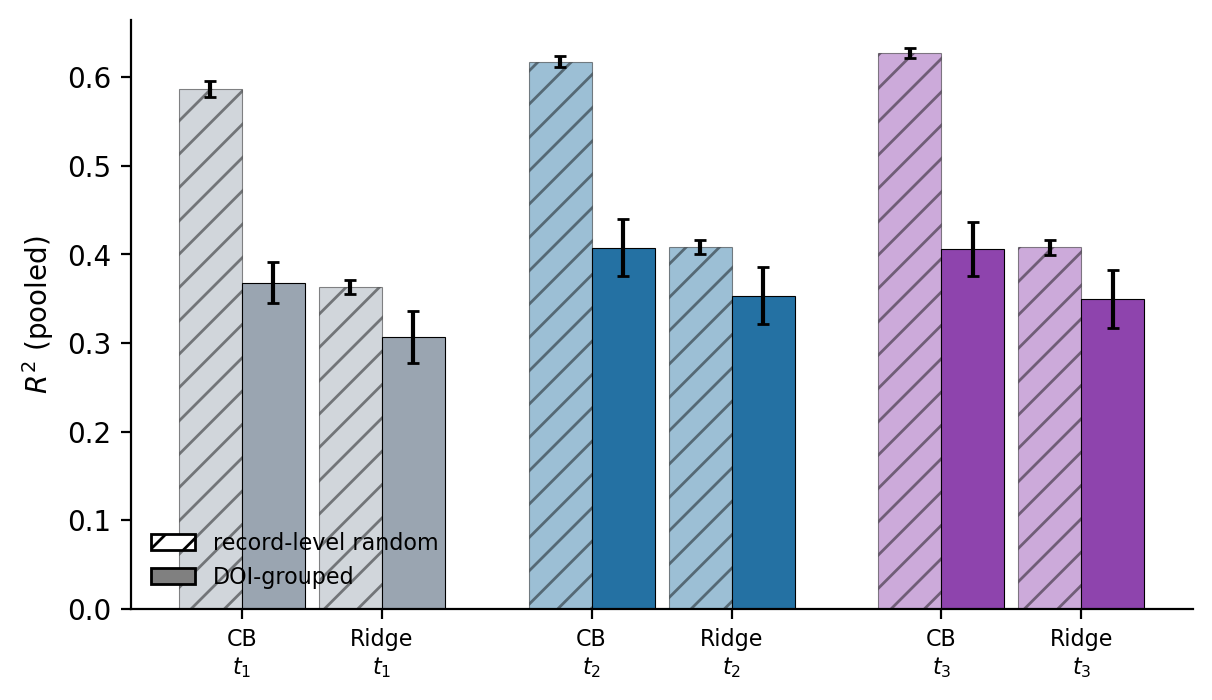
\includegraphics[width=0.6\textwidth]{figures/fig_split_effect.png}
\caption{Record-level random splits versus DOI-grouped splits for the three feature tiers (pooled dataset; mean $\pm$ s.d. over five splits).}
\label{fig:split}
\end{figure}

\subsection{Contribution of material-property and literature-derived features}

\subsubsection{Material-property descriptors.}
Adding material-property descriptors ($t_1 \rightarrow t_2$) increased $R^2$ by 0.038 (pooled), 0.065 (p-i-n) and 0.034 (n-i-p) and lowered MAE and RMSE in all three subsets (Table~\ref{tab:delta}), the largest gain between any two tiers. Because $t_1$ contains no explicit transport-layer material identities (Section~2.3.3), the $t_2$ descriptors convey both which materials were used and their reference properties. Each property is a fixed function of the material, so this gain is best interpreted as the value of encoding material choice through physically meaningful descriptors rather than as evidence that the specific property values themselves determine PCE. This is consistent with prior work showing that the representation of material and process information strongly affects PCE prediction \cite{fukasawa2024effectiveness}, and shows that the benefit persists when entire publications are held out.

\subsubsection{LLM-derived literature features.}
Adding LLM-derived literature features ($t_2 \rightarrow t_3$) under the same model configuration improved mean performance in every subset and every metric. Mean $R^2$ increased by 0.005 (pooled), 0.007 (p-i-n) and 0.006 (n-i-p); mean RMSE decreased by 0.015, 0.021 and 0.021 percentage points; and mean MAE also decreased in all three subsets (Table~\ref{tab:delta}). The individual gains are small relative to the material-property gain, and the standard deviations of the paired differences (0.006--0.007 in $R^2$) are comparable to the mean gains. However, the direction of the change was the same in all nine subset--metric combinations. \authortodo{report in how many of the five paired splits $t_3$ outperformed $t_2$ for each subset} Because the five repeated holdout splits have overlapping test sets, the paired differences are reported descriptively rather than with a formal significance test. The SHAP analysis (Section~\ref{sec:shap}) confirms that the fitted model uses the literature-derived features, although attribution indicates use of a feature rather than its predictive benefit.
% Optional control: append 44 random-noise columns to t2 and report their SHAP share and metric change, to show that the LLM group's ~4% attribution exceeds that of uninformative features.

\begin{table}[t]
\centering\small
\caption{Change in mean performance between feature tiers (paired per-split differences; s.d. of the five paired differences in parentheses).}
\label{tab:delta}
\begin{tabular}{lcccc}
\toprule
 & \multicolumn{2}{c}{$\Delta R^2$} & \multicolumn{2}{c}{$\Delta$RMSE (points)} \\
\cmidrule(lr){2-3}\cmidrule(lr){4-5}
Subset & $t_1\!\to\! t_2$ & $t_2\!\to\! t_3$ & $t_1\!\to\! t_2$ & $t_2\!\to\! t_3$ \\
\midrule
Overall & $+0.038\;(0.004)$ & $+0.004\;(0.006)$ & $-0.121\;(0.011)$ & $-0.015\;(0.020)$ \\
p-i-n   & $+0.065\;(0.013)$ & $+0.007\;(0.006)$ & $-0.184\;(0.034)$ & $-0.021\;(0.017)$ \\
n-i-p   & $+0.034\;(0.007)$ & $+0.006\;(0.007)$ & $-0.112\;(0.024)$ & $-0.021\;(0.024)$ \\
\bottomrule
\end{tabular}
\end{table}

\subsection{Interpretation of model predictions}
\label{sec:shap}

\subsubsection{Global importance.}
Perovskite quenching/crystallisation \authortodo{define this feature: source PDP column, categories and encoding} was the highest-ranked predictor in the pooled and n-i-p models (mean $|$SHAP$|$ 0.835 and 0.938 PCE percentage points) and second in the p-i-n model (0.461), where HTL band gap ranked first (0.535). In the pooled model the next features were HTL band gap (0.293), average perovskite atomic mass (0.292), total ion count (0.263), the missingness indicator of the perovskite photoluminescence maximum (0.219) and perovskite annealing time (0.218) (Fig.~\ref{fig:beeswarm}). Because material properties are fixed functions of material identity, layer-property features such as HTL band gap also act as identifiers of the material used in that layer. Aggregating importance by feature group (Fig.~\ref{fig:groups}) shows that process variables and material-property descriptors dominate, followed by composition descriptors.

The 44--46 literature-derived features account for 3.9\% (pooled), 4.1\% (p-i-n) and 3.5\% (n-i-p) of the total absolute SHAP attribution, showing that the fitted models use this information alongside the database, composition, and material-property descriptors. The highest-ranked literature-derived feature in all three models was \texttt{json\_numeric\_values\_found}, the number of numerical values recovered from a paper (ranked 28th, 23rd and 32nd in the pooled, p-i-n and n-i-p models). This descriptor reflects how completely a publication reports its experimental details rather than a specific material or processing parameter. It was followed by the presence of a passivation layer (52nd, pooled).

\begin{figure}[t]
\centering
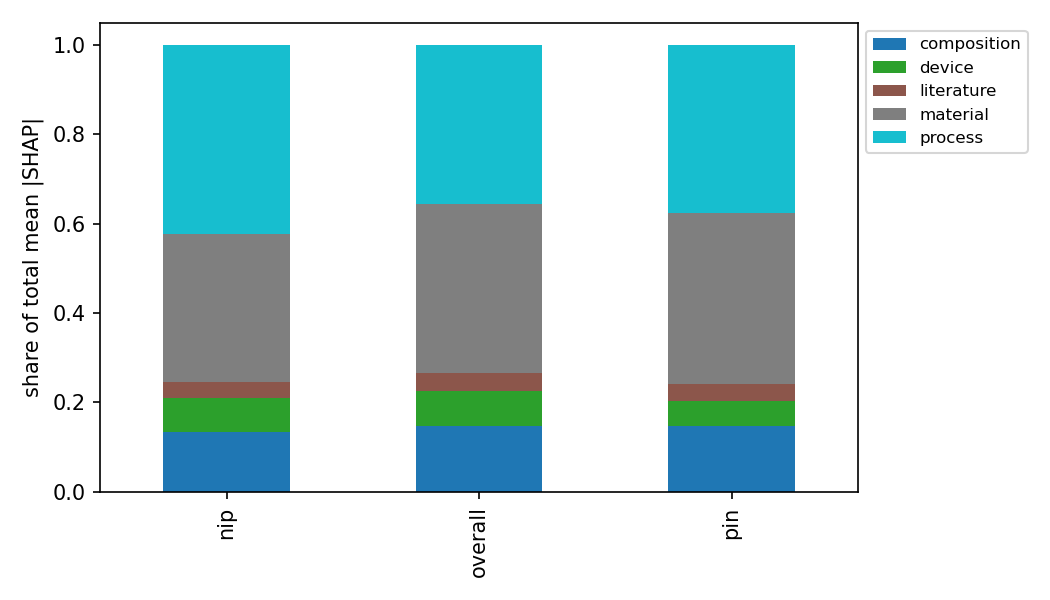
\includegraphics[width=\textwidth]{figures/fig_shap_groups.png}
\caption{Share of total feature attribution by feature group for the $t_3$ CatBoost models. Bar lengths are group-summed mean absolute SHAP values as a percentage of the model total $\Sigma$ (6.79 Overall, 5.33 p-i-n, 6.65 n-i-p). Units throughout are PCE percentage points; $\Sigma$ is the sum of mean $|\mathrm{SHAP}|$ over all features (223/225/221 per model). Process and material-property groups dominate every architecture, while LLM-derived literature features contribute 3.5--4.1\%.}
\label{fig:groups}
\end{figure}

\subsubsection{Architecture-specific associations.}
For p-i-n devices, the highest-ranked features were HTL band gap (0.535), perovskite quenching/crystallisation (0.461), ETL deposition method (0.400), HTL LUMO (0.346), Pb fraction (0.268), perovskite thickness (0.233) and annealing time (0.195). For n-i-p devices, quenching/crystallisation (0.938) was followed by average perovskite atomic mass (0.471), HTL deposition method (0.292), annealing time (0.211), average perovskite radius (0.201), the missingness indicator of the perovskite photoluminescence maximum (0.200) and ETL deposition method (0.196). Because the two models were fitted to different records, these differences describe learned associations, not differences in physical effects between architectures, and SHAP values do not establish causal effects.

\begin{figure}[p]
\centering
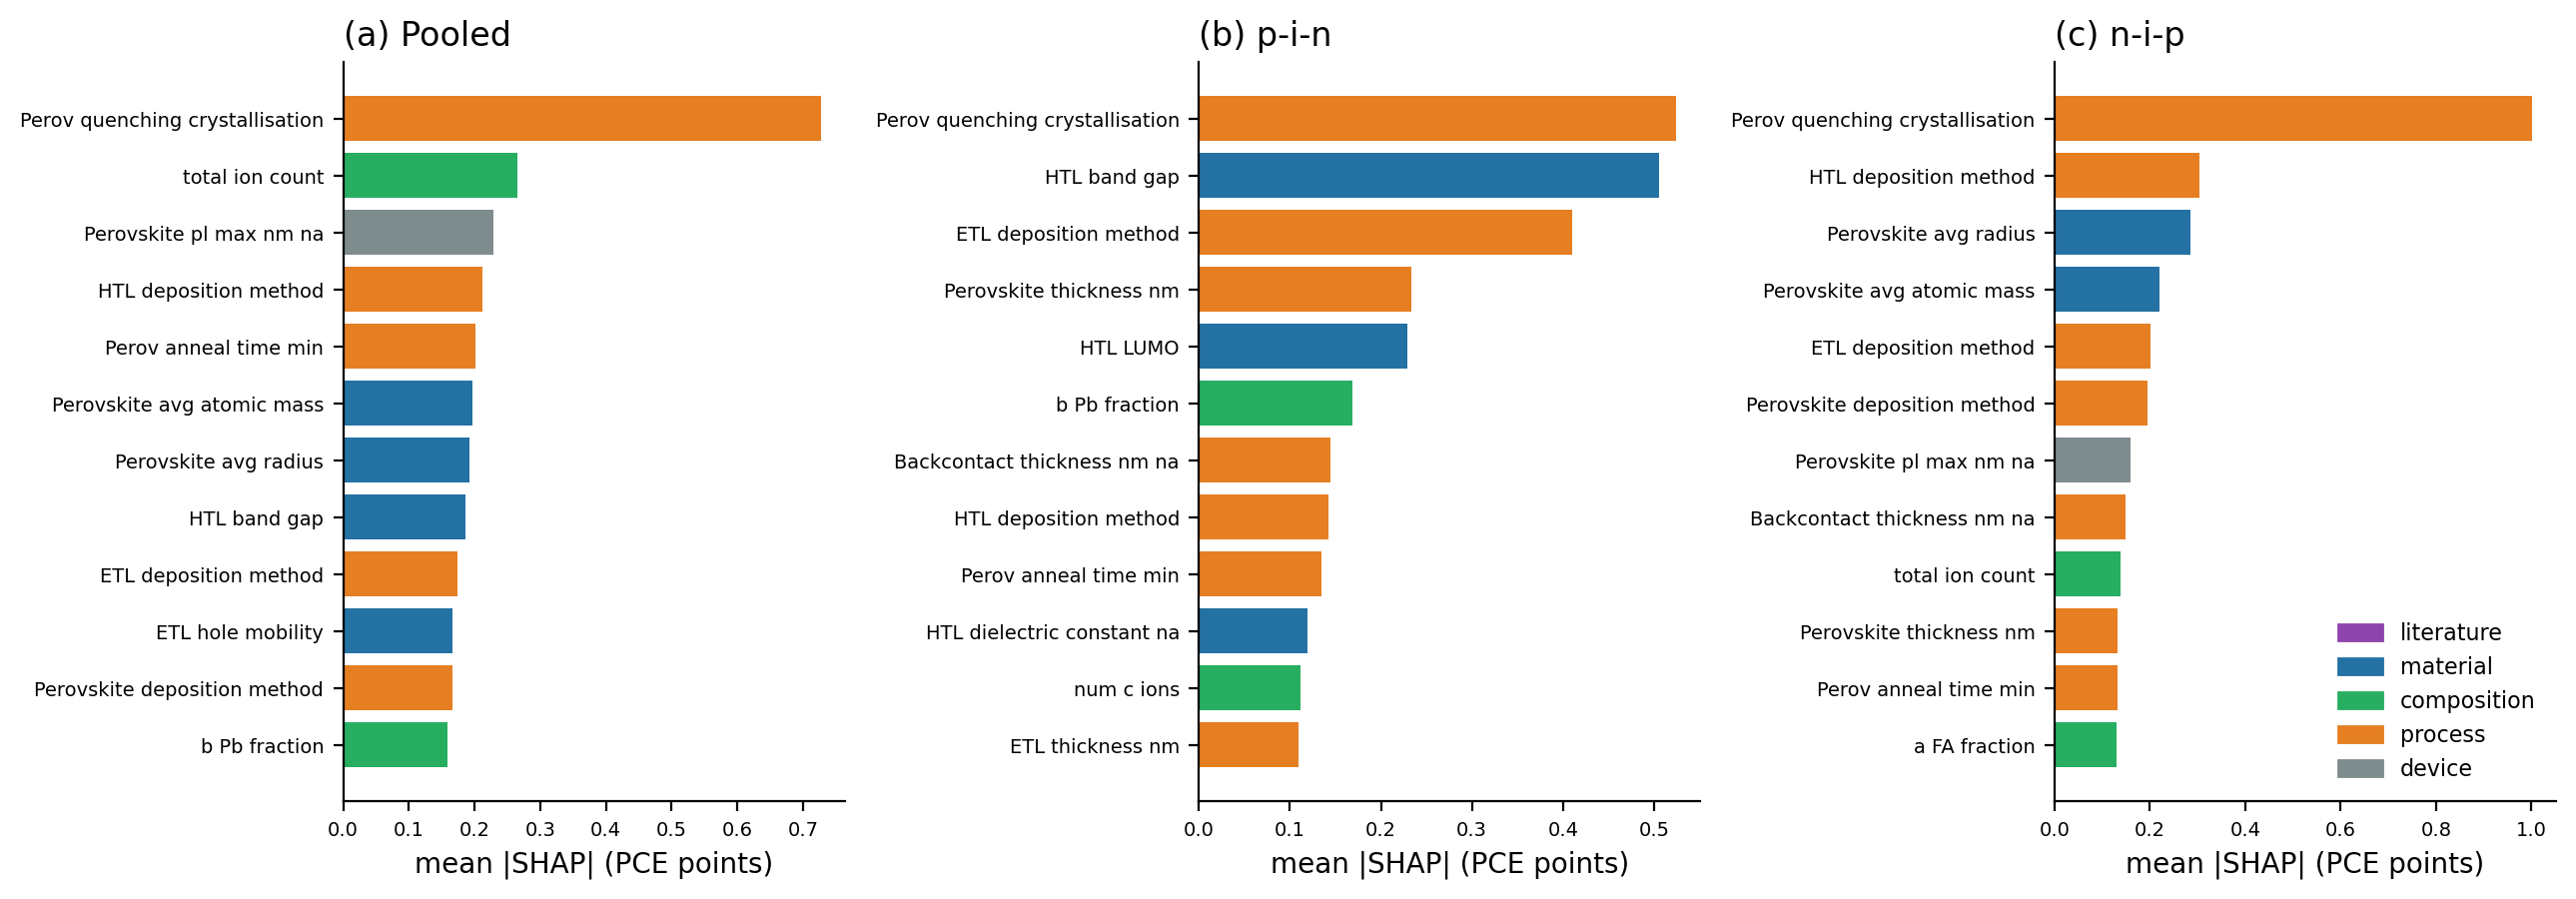
\includegraphics[width=0.9\textwidth]{figures/shap.png}
\caption{Mean $|$SHAP$|$ of the ten highest-ranked features within the material-property (top row) and process-parameter (bottom row) feature groups for the pooled, p-i-n and n-i-p models (first DOI-grouped split). Units are PCE percentage points; \texttt{\_na} denotes a missingness indicator.
\authortodo{regenerate from the final $t_3$ CatBoost model: plotted values do not match the text (e.g.\ pooled quenching 0.801 vs 0.835; n-i-p average atomic mass 0.199 vs 0.471); move \texttt{json\_numeric\_values\_found} out of the p-i-n process panel into the literature group; enlarge fonts}}
\label{fig:beeswarm}
\end{figure}

\subsection{Comparison with previous PDP-based studies}

To place the framework relative to previous PDP-based work, we adapted the publicly available pipelines of Roberts et al.\ and Fukasawa et al.\ \cite{roberts2024machine,fukasawa2024effectiveness} to PCE prediction and evaluated them on the same DOI-grouped test records as our model (Table~\ref{tab:previous_pdp_studies}). The reported metrics come from our runs of these implementations and differ from the values reported in the original publications, which used a different target (Roberts et al., $J_{\mathrm{SC}}$) or record-level and temporal test sets (Fukasawa et al.).

On the first DOI-grouped split, the Roberts-based pipeline (XGBoost with its feature encoding, default hyperparameters) reached $R^2 = 0.368$ and MAE $= 2.98$ percentage points, compared with $R^2 = 0.403$ and MAE $= 2.92$ for our $t_3$ CatBoost model on the same 8,395 test records. \authortodo{confirm that the Roberts duplicate-averaging step was applied to training records only, so that both models are scored on the identical 8,395 test records; extend both comparisons to all five splits and report mean $\pm$ s.d.}

\authortodo{Fukasawa-based benchmark (Random Forest, 1st split with zero complement, Oliynyk composition vectors): report $R^2$ and MAE on the same split(s) and add one or two sentences of discussion.} Fukasawa et al.\ reported $R^2 = 0.45$ and MAE $= 3.20\%$ on 294 newly registered records \cite{fukasawa2024effectiveness}; because that test set differs in size, composition and time period from the DOI-grouped partitions used here, those values are not directly comparable with Table~\ref{tab:previous_pdp_studies}.

\begin{table}[t]
\centering
\small
\caption{Comparison with benchmark implementations adapted from the public codebases of Roberts et al.\ and Fukasawa et al., evaluated on the first DOI-grouped split ($n = 8{,}395$ test records) with PCE as the target. Metrics are from our runs of these implementations, not the original publications. MAE in PCE percentage points.}
\label{tab:previous_pdp_studies}
\begin{tabular}{llcc}
\toprule
Implementation & Model configuration & $R^2$ & MAE \\
\midrule
This study ($t_3$) & CatBoost & 0.403 & 2.92 \\
Roberts-based pipeline & XGBoost, default hyperparameters & 0.368 & 2.98 \\
Fukasawa-based pipeline & Random Forest & \authortodo{} & \authortodo{} \\
\bottomrule
\end{tabular}
\end{table}

\subsection{Limitations}
Results come from a single database with heterogeneous reporting. The DOI-grouped holdout measures generalization to unseen publications, but the five repeated test sets overlap, so the reported uncertainties are not those of an independent repeated grouped cross-validation. Grouping by DOI does not separate publications from the same research group, which may share materials and recipes across papers; grouping by corresponding author or laboratory, and a temporal split that trains on earlier publications and tests on later ones, would give stricter estimates of generalization. LLM-derived features were available for 36.2\% of the records, and the extraction quality bounds the information these features can carry. Literature features are defined per publication and therefore cannot distinguish between devices within the same paper. SHAP rankings are associative. Predictions saturate near 21\% PCE, and devices with reported PCE below 1\% were excluded.

% ---------------- CONCLUSION ----------------
\section{Conclusion}
We developed a literature- and material-augmented machine-learning framework for predicting the power conversion efficiency of perovskite solar cells and evaluated it on unseen publications using DOI-grouped holdout splits. The work makes two contributions. First, augmenting the PDP database representation improves prediction on unseen publications: with a fixed CatBoost configuration, material-property descriptors gave the largest gain ($\Delta R^2 = +0.038$ pooled), and LLM-derived literature features extracted from 2,726 full-text articles gave a further small improvement in every architecture subset and every error metric ($\Delta R^2 = +0.005$ to $+0.007$). The final model reached a pooled $R^2$ of 0.413 (MAE 2.91 percentage points), with $R^2$ of 0.365 for p-i-n and 0.452 for n-i-p devices. Second, publication-level evaluation is necessary for realistic estimates on literature-derived data: record-level random splitting overestimated $R^2$ by 0.17--0.24, and the overestimate was largest for the literature-augmented model, whose apparent gain from LLM features was 0.074 under random splits but 0.004 under DOI-grouped splits. We therefore recommend DOI-grouped (or stricter) evaluation as the default for machine learning on the Perovskite Database and similar literature-compiled datasets.

\bibliographystyle{elsarticle-num}
\bibliography{references}

\end{document}